\chapter{Evaluation und Validation}
\label{ch:Eval}

Um das System zu validieren und die Grenzen der Infrarotbildverarbeitung in diesem Gebiet zu ermitteln wurden einige Experimente durchgeführt. Diese Experimente zeigen, was das System kann und wo die Grenzen des Systems und auch der Infrarottechnik liegen.\\
\\
Zur Auswertung der Experimente werden Bilder mit Markierungen verwendet. Diese sind wie folgt Farbcodiert.

\begin{itemize}
	\item Grün -> Korrekt gefundene Person (True Positive)
	\item Gelb -> Nicht gefundene Person (False Negative)
	\item Rot -> Nichtiger Treffer (False Positive)\\
\end{itemize}
Zudem werden die folgenden Metriken verwendet, diese sind leicht angepasst, da die Klasse True Negative fehlt:

\begin{itemize}
	\item Accuracy: \[\dfrac{TP}{Anzahl\: moegliche\: Treffer}\]
	\item Precision: \[\dfrac{TP}{TP + FP}\]
	\item Recall: \[\dfrac{TP}{TP + FN}\]
	\item F1-Score: \[\dfrac{2*Precision*Recall}{Precision + Recall}\]
\end{itemize}


\section{Vergleich mit Anforderungen}
\label{sec:VergleichAnforderungen}

Die Aufgabe war es, ein System zu entwickeln, welches in dem Sitzungszimmer auf den Bildern der Infrarotkameras die Anzahl und Position der Personen ermittelt. Dieser Punkt wurde erfüllt. Das System kann dynamisch Personen und deren Position ermitteln und diese ausgeben. Das System zeigte bei den Tests wie in Abbildung \ref{fig:ExperimentSummary} zu sehen eine Precision Score von 97\% das bedeutet, dass es fast gar keine False Positiv Treffer gab. Die Accuracy liegt nur bei 85\%, dies weil in den Experimenten auch die Grenzen der Personenerkennung getestet werden wie in Kapitel \ref{sec:cloths} diskutiert wird.

\begin{figure}[H]
	\centering
	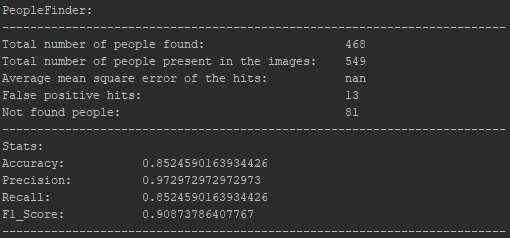
\includegraphics[width=.9\linewidth]{ExperimentSummary}
	\caption{Zusammenfassung aller ergebnisse der Experimente}
	\label{fig:ExperimentSummary}
\end{figure}



\section{Fremde Wärmequellen}
\label{sec:FremdeWärmequellen}

In diesem Versuch wurde der Einfluss von fremden Wärmequellen, wie zum Beispiel Laptops, Natels, oder Kaffees, evaluiert. Dabei wurde der Effekt von Störquellen mit und ohne Personen im Raum analysiert.

\subsection{Versuchsaufbau}

Um die Performance der Algorithmen spezifisch in Bezug auf fremde Wärmequellen zu testen, wurden verschiedene Testsituationen erzeugt. Zuerst wurden fünf Laptops, von 13" bis 17",auf den Sitzungstisch gestellt, um zu sehen, ob Laptops ohne Personen Treffer generieren. Die Geräte wurden auf den gesamten Kamerawinkel verteilt, vom Zentrum des Bildes bis an den Rand. Da die Algorithmen nicht durch die Anzahl Wärmequellen, sondern nur durch die Distanz zwischen den Wärmequellen beeinflusst werden, konnte der ganze Kamerawinkel in einem einzigen Versuch getestet werden.\\
Die Laptops waren seit ca. 1.5h in leichtem Betrieb, ihre Temparatur war ca. 25\degree C, somit leicht diese etwas unter der Abstrahlungswärme einer Person. Die Hauttemperatur einer Person wird von den Infrarotkameras zwischen 27\degree C und 33\degree C gemessen, je nach Kleidung und Behaarung.\\
Danach nahmen fünf Personen bei den Laptops platz,  ohne dass die Laptops verschoben wurde. Um zu testen, ob False Positives generiert werden, wenn jemand den Laptop bedient, die Arme zum Laptop reichen.\\
Um auch Wärmere Laptops überprüfen zu können wurde Bilder während einer Besprechung aufgezeichnet. Dabei war ein Laptop, dessen Temperatur im Bereich der Hauttemperatur einer Person liegt, in der Mitte des Tischs. Die szene sah, wie in Abbildung \ref{fig:groundDeviceTest2} zu sehen, aus.
\\
\begin{figure}[H]
	\centering
	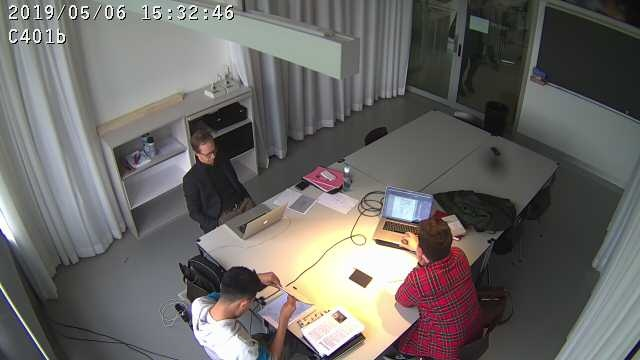
\includegraphics[height=4cm]{groundDeviceTest2}
	\caption{Ansicht des Sitzungszimmers während der aufnahme des zusätzlichen Laptop und Personen Testsets}
	\label{fig:groundDeviceTest2}
\end{figure}
Schon bei der Erstellung der Modelle wurde ersichtlich, dass das Herausfiltern von Wärmequellen mit sehr kleiner Fläche für beide Algorithmen kein Problem darstellt. Aus diesem Grund wurden die Versuche mit kleineren Wärmequellen nur in kleinem Rahmen durchgeführt. Es wurde Test mit einem Mobiltelefon durchgeführt, in dem ein Natel an verschiedenen Postionen auf den Tisch gelegt wurde. Da Mobiltelefone meist in der Hosentasche getragen werden, weisen diese Temperaturen bis zu 34\degree C auf.\\
\\

\subsection{Resultate}

\begin{table}[H]
	\begin{tabularx}{\textwidth}{|X|X|X|X|}
		\hline
		\textbf{\gls{CNN} Ergebnisse Fremde Wärmequellen} & \textbf{Nur Laptops} & \textbf{Laptops mit Personen} & \textbf{Mobiltelefon}\\
		\hline 
		\textbf{Gesamtanzahl Personen in Bilder} & 0 & 94 & 0\\
		\hline
		\textbf{Korrekt identifizierter Personen} & 0 & 85 & 0 \\
		\hline
		\textbf{Falsche Treffer} & 2 & 12 & 0 \\
		\hline
		\textbf{Nicht erkannte Personen} & 0 & 9 & 0\\
		\hline
		\textbf{Accuracy} & - & 90\% & -\\
		\hline  
		\textbf{Precision} & 0\% & 87\% & 100\%\\
		\hline
		\textbf{F1-Score} & - & 89\% & - \\
		\hline
	\end{tabularx}
	\caption{Ergebnisse des \gls{CNN}, der Experimente mit fremden Wärmequellen}
	\label{tbl:heatSources}
\end{table}

\begin{table}[H]
	\begin{tabularx}{\textwidth}{|X|X|X|X|X|}
		\hline
		\textbf{Threshold Ergebnisse Fremde Wärmequellen} & \textbf{Nur Laptops} & \textbf{Laptops mit Personen} & \textbf{Mobiltelefon} & \textbf{Essen}\\
		\hline 
		\textbf{Anzahl Personen im Bild} & wenig & wenig & 0 & ..\\
		\hline
		\textbf{Korrekt identifizierter Personen} & gross & 0 &..\\
		\hline
		\textbf{Falsche Treffer} & gross & 7 &..\\
		\hline
		\textbf{Nicht erkannte Personen} & gross & 0 &..\\
		\hline
		\textbf{Accuracy} & 93\% & \textasciitilde 1m & \textasciitilde 4-5m & ..\\
		\hline  
		\textbf{Precision} & passiv & passiv & passiv oder aktiv & ..\\
		\hline
		\textbf{F1-Score} & langsam & langsam & .. & ..\\
		\hline
	\end{tabularx}
	\caption{Ergebnisse der Threshold-Methode, der Experimente mit fremden Wärmequellen}
	\label{tbl:threshHeatSources}
\end{table}

\subsection{Evaluation}

Die Threshold-Methode kann, wie erwartet, nicht gut mit anderen Wärmequellen umgehen. Dies, weil die Threshold-Methode nur durch Temperatur und Mindestgrösse eines Objekts entscheiden kann, ob es sich um eine Person handelt oder nicht. Deshalb hatte dieser auf den Testbildern mit einer Person und einem Laptop, nur eine Precision Score von 64\% erreicht (Siehe Abbildung \ref{fig:ThreshPersonLaptop}).\\
\\
Das \gls{CNN} kann sehr gut mit anderen Wärmequellen umgehen, solange diese in ähnlicher Form antrainiert wurden. Dabei hilft es, dass in einem Sitzungszimmer nicht viele unterschiedliche Wärmequellen vorkommen können. \\
Die momentane Version des \gls{CNN}'s identifiziert teilweise grössere Laptops als Personen, wenn sie sich in einem ähnlichen Wärmebereich wie Personen befinden. Dieses Problem könnte, wie im Kapitel \ref{ch:Ausblick} noch diskutiert wird, durch verbesserte Trainingsdaten eliminiert werden.

\vspace{.5em}
\begin{figure}[H]
	\begin{subfigure}{.45\linewidth}
		\centering
		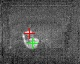
\includegraphics[keepaspectratio,height=4cm]{ThreshPersonLaptop}
		\caption{Ergebnis der Threshold-Methode des Experiments mit Laptop und Person}
		\label{fig:ThreshPersonLaptop}
	\end{subfigure}\hfill%
	\begin{subfigure}{.45\linewidth}
		\centering
		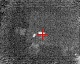
\includegraphics[keepaspectratio,height=4cm]{ThresholdLaptop}
		\caption{Threshold-Methode Ergebnis des Experiments mit nur einem Laptop}
		\label{fig:thresholdLaptop}
	\end{subfigure}
\begin{subfigure}{.45\linewidth}
	\centering
	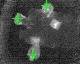
\includegraphics[keepaspectratio,height=4cm]{cnnPersonLaptop}
	\caption{\gls{CNN} Ergebnis des Experiments mit Laptop und Person}
	\label{fig:cnnPersonLaptop}
\end{subfigure}
	\begin{subfigure}{.55\linewidth}
		\centering
		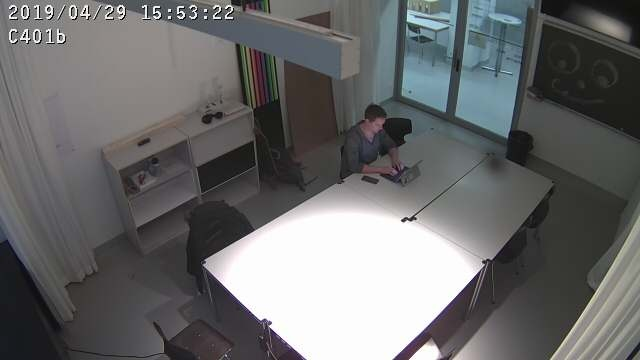
\includegraphics[keepaspectratio,height=4cm]{GroundHeatSources}
		\caption{Ground-Truth des Experiments mit Laptop und Person}
		\label{fig:groundPersonLaptop}
	\end{subfigure}
	\caption{Experimente mit fremden Wärmequellen}
	\label{fig:HeatSources}
\end{figure}
\vspace{.5em}



\section{Distanz}
\label{sec:distanz}

Die Distanz zwischen zwei Personen ist ein wichtiger Faktor, der sich gleichermassen auf die Threshold-Methode auswirkt, wie auch auf das \gls{CNN}. Da bei dem \gls{CNN} mit einer Sliding-Window Methode und Clustern der Treffer gearbeitet wird, kann das System, bei Personen, welche zu wenig Abstand zueinander haben, nicht mehr zwischen den Treffern unterscheiden. Bei der Threshold-Methode wird die Silhouette der Personen leicht vergrössert, wodurch mehrere Personen bei geringem Abstand als einzelner Treffer gewertet werden.

\subsection{Versuchsaufbau}

Es wurden vier Personen in zwei Paaren so platziert, dass sich das eine Paar in einem idealen Winkel zur Infrarotkamera aufhält und das andere Paar in einem möglichst schwierigen Winkel. Dies ist in Abbildung \ref{fig:cnnDistance10} gut zu sehen. Zwei Personen sind deutlich voneinander getrennt, die anderen zwei überlappen sich auf Grund des Kamerawinkels. Dieses Setting wurde gewählt, um in einem Test beide Extreme überprüfen zu können. 
Beim Test wurde schrittweise der Abstand zwischen den Testpersonen erhöht, um festzustellen, ab welcher Distanz die Algorithmen erfolgreich die Personen erkennen. Der Abstand wird in 10cm Schritten erhöht, weil 10cm auf Tischhöhe ca. einem Pixel auf dem Bild entspricht.

\subsection{Resultate}

\begin{table}[H]
	\begin{tabularx}{\textwidth}{|X|X|X|X|X|}
		\hline
		\textbf{Ergebnisse Distanztest} & \textbf{10cm} & \textbf{20cm} & \textbf{30cm} & \textbf{40cm}\\
		\hline 
		\textbf{Accuracy} & 93\% & \textasciitilde 1m & \textasciitilde 4-5m & ..\\
		\hline  
		\textbf{Precision} & passiv & passiv & passiv oder aktiv & ..\\
		\hline
		\textbf{F1-Score} & langsam & langsam & .. & ..\\
		\hline
		\textbf{Interferenz durch Wasser und Metal} & wenig & wenig & viel & ..\\
		\hline
		\textbf{Grösse der Tags} & gross & gross & klein & ..\\
		\hline
	\end{tabularx}
	\caption{Ergebnisse des Distanztests}
	\label{tbl:distance}
\end{table}

\subsection{Evaluation}

Die Algorithmen können Personen bereits ab einem Abstand von 10cm auseinanderhalten, sofern die Personen so ausgerichtet sind, dass die optische Verzerrung keinen Einfluss auf den Zwischenraum hat. Wie in den Abbildungen in der linken Bildhälfte zu sehen ist, können die Personen, die auf die Kamera ausgerichtet sind, unterschieden werden. Sind die Person jedoch so platziert, wie auf der rechten Bildhälfte zu sehen ist, sind diese von der Kamera aus gesehen, hintereinander. Bei so kleinen Abstand kann der Algorithmus deshalb nicht mehr herausfiltern, ob es sich um eine oder mehrere Personen handelt.\\
\\
Befinden sich die Personen in der schlechtest möglichen Position, benötigen die Algorithmen einen Mindestabstand von 30cm, um die Personen fehlerfrei unterscheiden zu können. Siehe Abbildungen \ref{fig:cnnDistance30} und \ref{fig:thresholdDistance30}

\begin{figure}[H]
	\begin{subfigure}{.45\linewidth}
		\centering
		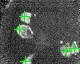
\includegraphics[keepaspectratio,height=4cm]{CNNDistance10}
		\caption{\gls{CNN} Ergebnis des Distanztest mit 10cm Abstand}
		\label{fig:cnnDistance10}
	\end{subfigure}\hfill%
	\begin{subfigure}{.45\linewidth}
		\centering
		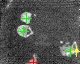
\includegraphics[keepaspectratio,height=4cm]{ThresholdDistance10}
		\caption{Threshold Ergebnis des Distanztest mit 10cm Abstand}
		\label{fig:thresholdDistance10}
	\end{subfigure}
	\begin{subfigure}{\linewidth}
		\centering
		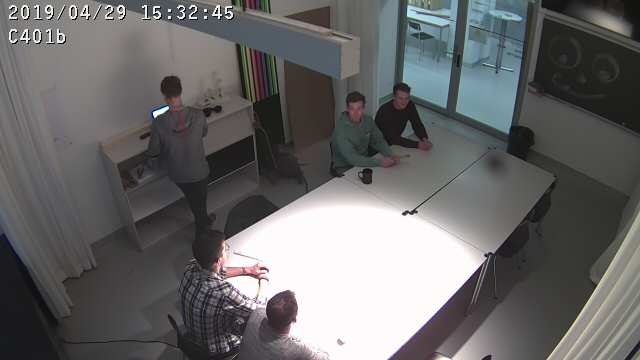
\includegraphics[keepaspectratio,height=3cm]{GroundDistance10}
		\caption{Ground-Truth Distanzexperiment mit 10cm Abstand}
		\label{fig:groundDistance10}
	\end{subfigure}
	\caption{Distanzexperiment 10cm}
	\label{fig:Distance10}
\end{figure}

\begin{figure}[H]
	\begin{subfigure}{.45\linewidth}
		\centering
		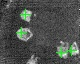
\includegraphics[keepaspectratio,height=4cm]{CNNDistance30}
		\caption{\gls{CNN} Ergebnis des Distanztest mit 30cm Abstand}
		\label{fig:cnnDistance30}
	\end{subfigure}\hfill%
	\begin{subfigure}{.45\linewidth}
		\centering
		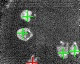
\includegraphics[keepaspectratio,height=4cm]{ThresholdDistance30}
		\caption{Threshold Ergebnis des Distanztest mit 30cm Abstand}
		\label{fig:thresholdDistance30}
	\end{subfigure}
	\begin{subfigure}{\linewidth}
		\centering
		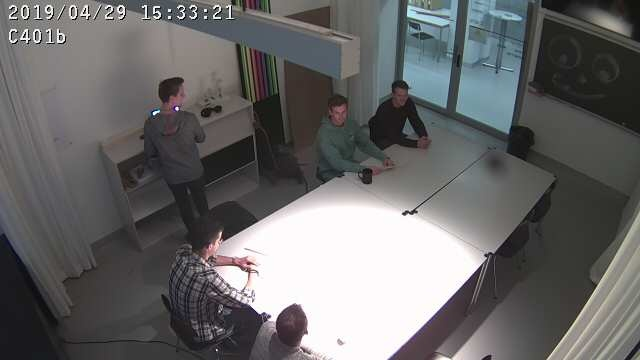
\includegraphics[keepaspectratio,height=3cm]{GroundDistance30}
		\caption{Ground-Truth}
		\label{fig:groundDistance30}
	\end{subfigure}
	\caption{Distanzexperiment 30cm}
	\label{fig:Distance30}
\end{figure}

\section{Grösse Des Objekts auf dem Bild}
\label{sec:objectSize}
Eine Spezialität des Sitzungszimmers, das zur Verfügung gestellt wurde, ist, dass die Höhe der Decke verändert werden kann. Da die Infrarotkameras an der Decke montiert sind, wurde dies als Möglichkeit genutzt um zu testen wie die Algorithmen auf grössen der Objekte im Bild reagieren. 

\subsection{Versuchsaufbau}

Die verstellbare Decke des Sitzungszimmers wurde auf die vom Mobiliar zugelassene Minimalhöhe, ca. 255cm, heruntergefahren. Danach wurden wiederum Infrarotbilder von Testpersonen aufgenommen. Anschliessend wurde die Decke maximal hochgefahren, etwa 400cm, und noch einmal Bilder aufgezeichnet.

\subsection{Resultate}

\begin{table}[H]
	\begin{tabularx}{\textwidth}{|X|X|X|X|X|}
		\hline
		\textbf{Ergebnisse des Objektgrössenexperiments} & \textbf{255cm} & \textbf{400cm} & \textbf{30cm} & \textbf{40cm}\\
		\hline 
		\textbf{Accuracy} & 93\% & \textasciitilde 1m & \textasciitilde 4-5m & ..\\
		\hline  Precision
		\textbf{Precision} & passiv & passiv & passiv oder aktiv & ..\\
		\hline
		\textbf{F1-Score} & langsam & langsam & .. & ..\\
		\hline
		\textbf{Interferenz durch Wasser und Metal} & wenig & wenig & viel & ..\\
		\hline
		\textbf{Grösse der Tags} & gross & gross & klein & ..\\
		\hline
	\end{tabularx}
	\caption{Ergebnisse des Distanztests}
	\label{tbl:distance}
\end{table}

\subsection{Evaluation}
Beide Algorithmen können mit der getesteten Reichweite von Objektgrössen 
Beide Algorithmen können sehr gut mit dem Verstellen der Decke umgehen. Das einzige Problem ist, dass umso tiefer die Decke eingestellt ist, umso kleiner ist die Fläche im Raum, die von den Infrarotkameras aufgenommen wird. Anderweitig hat die Deckenhöhe keinen Einfluss auf die Algorithmen.\\
Möchte man jedoch die reale Position der Personen aus dem Bild berechnen, müsste die Deckenhöhe zusätzlich berechnet oder gemessen werden.

\begin{figure}[H]
	\begin{subfigure}{.45\linewidth}
		\centering
		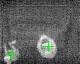
\includegraphics[keepaspectratio, height=4cm]{cameraHeightLow}
		\caption{Ergebnis des \gls{CNN} mit Deckenhöhe 255cm}
		\label{fig:cameraHeightLow}
	\end{subfigure}
	\begin{subfigure}{.45\linewidth}
		\centering
		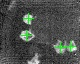
\includegraphics[keepaspectratio, height=4cm]{cameraHeightHigh}
		\caption{Ergebnis des \gls{CNN} mit Deckenhöhe 400cm}
		\label{fig:cameraHeightHigh}
	\end{subfigure}
\end{figure}


\section{Kleider}
\label{sec:cloths}

Infrarotbilder zeigen die Wärmeabstrahlung der verschiedenen Objekte im Bild. Wird eine Wärmequelle isoliert, verschwindet sie auf dem Infrarotbild. Genau das passiert, wenn stark isolierende Kleider getragen werden. Da in dieser Arbeit die Vogelperspektive analysiert wird, haben vor allem Kopfbedeckungen, Schals und Jacken einen grossen Einfluss. 

\subsection{Versuchsaufbau}

Eine Testperson hielt sich im Raum auf und trug verschiedene Kleidungsstücke. Dabei wurden eine Mütze, ein Schal und eine Jacke einzeln und in allen möglichen Kombinationen von der Testperson getragen.

\subsection{Evaluation}
Kleider beeinflussen die Performance der Algorithmen massiv. Trägt eine Person z.B. eine Mütze, wird sie vom \gls{CNN} noch zu 80\% erkannt. Bei der Threshold-Methode sind es 76\%. Zudem kann es dazu führen, dass eine Person zwei Treffer erzeugt (siehe Abbildung \ref{fig:thresholdClothHat}).\\
\\
Wenn ein Schal getragen wird, sinkt die Accuracy auf ca. 60\% bei beiden Algorithmen. Betrachtet man Abbildung \ref{fig:scarfIR} sieht man deutlich, wie der Schal einen Teil der Wärme der Person verdeckt.\\
\\
Das Tragen einer Jacke macht es für die Algorithmen beinahe unmöglich die Personen zu erkennen. Die Person wird nur noch in wenigen Fällen erkannt. Das \gls{CNN} könnte wahrscheinlich mit den entsprechenden Trainingsdaten erweitert werden, sodass auch diese Personen erkannt werden. Da aber die Fläche der Abwärme einer Person so nur noch wenige Pixel beträgt, wird es schwieriger diese von fremden Wärmequellen zu unterscheiden.\\

\begin{figure}[H]
	\begin{subfigure}{.45\linewidth}
		\centering
		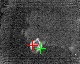
\includegraphics[keepaspectratio, height=4cm]{thresholdClothHat}
		\caption{Resultat der Threshold-Methode des Experiments mit Kopfbedeckung}
		\label{fig:thresholdClothHat}
	\end{subfigure}
	\begin{subfigure}{.45\linewidth}
		\centering
		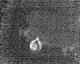
\includegraphics[keepaspectratio, height=4cm]{scarfIR}
		\caption{Infrarotbild einer Person die einen Schal trägt}
		\label{fig:scarfIR}
	\end{subfigure}
	
\end{figure}

Die Tests zeigen schon bei der manuellen, visuellen Analyse der Abbildung \ref{fig:rawClothAll}, dass wenn Jacke, Mütze und Schal zusammen getragen werden, man die Person nicht mehr erkennen kann.

\begin{figure}[H]
	\begin{subfigure}{.45\linewidth}
		\centering
		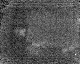
\includegraphics[keepaspectratio, height=4cm]{rawClothAll}
		\caption{Infrarotbild des Experiments mit Jacke, Mütze und Schal}
		\label{fig:rawClothAll}
	\end{subfigure}
	\begin{subfigure}{.45\linewidth}
		\centering
		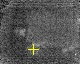
\includegraphics[keepaspectratio, height=4cm]{clothAll}
		\caption{Position der Person}
		\label{fig:AlgorithmsClothAll}
	\end{subfigure}
	\begin{subfigure}{\linewidth}
		\centering
		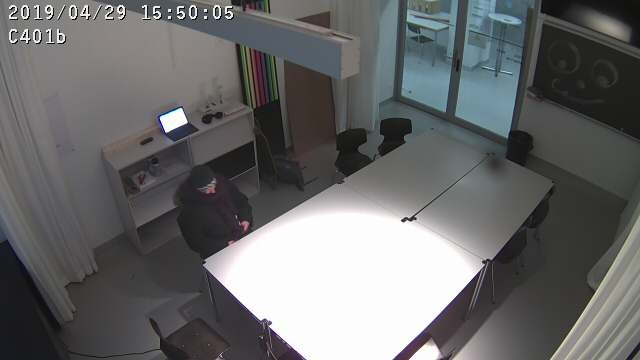
\includegraphics[keepaspectratio, width=.5\linewidth]{GroundClothAll}
		\caption{Ground-Truth des Experiments mit allen Kleidern}
		\label{fig:groundTruthClothAll}
	\end{subfigure}
	\caption{Experiment mit Jacke Mütze und Schal}
	\label{fig:AllCloth}
\end{figure}

